\documentclass[]{article}
\usepackage{lmodern}
\usepackage{amssymb,amsmath}
\usepackage{ifxetex,ifluatex}
\usepackage{fixltx2e} % provides \textsubscript
\ifnum 0\ifxetex 1\fi\ifluatex 1\fi=0 % if pdftex
  \usepackage[T1]{fontenc}
  \usepackage[utf8]{inputenc}
\else % if luatex or xelatex
  \ifxetex
    \usepackage{mathspec}
  \else
    \usepackage{fontspec}
  \fi
  \defaultfontfeatures{Ligatures=TeX,Scale=MatchLowercase}
\fi
% use upquote if available, for straight quotes in verbatim environments
\IfFileExists{upquote.sty}{\usepackage{upquote}}{}
% use microtype if available
\IfFileExists{microtype.sty}{%
\usepackage{microtype}
\UseMicrotypeSet[protrusion]{basicmath} % disable protrusion for tt fonts
}{}
\usepackage[margin=1in]{geometry}
\usepackage{hyperref}
\hypersetup{unicode=true,
            pdftitle={The Guardian Knowledge June 2019},
            pdfauthor={Robert Hickman},
            pdfborder={0 0 0},
            breaklinks=true}
\urlstyle{same}  % don't use monospace font for urls
\usepackage{color}
\usepackage{fancyvrb}
\newcommand{\VerbBar}{|}
\newcommand{\VERB}{\Verb[commandchars=\\\{\}]}
\DefineVerbatimEnvironment{Highlighting}{Verbatim}{commandchars=\\\{\}}
% Add ',fontsize=\small' for more characters per line
\usepackage{framed}
\definecolor{shadecolor}{RGB}{248,248,248}
\newenvironment{Shaded}{\begin{snugshade}}{\end{snugshade}}
\newcommand{\AlertTok}[1]{\textcolor[rgb]{0.94,0.16,0.16}{#1}}
\newcommand{\AnnotationTok}[1]{\textcolor[rgb]{0.56,0.35,0.01}{\textbf{\textit{#1}}}}
\newcommand{\AttributeTok}[1]{\textcolor[rgb]{0.77,0.63,0.00}{#1}}
\newcommand{\BaseNTok}[1]{\textcolor[rgb]{0.00,0.00,0.81}{#1}}
\newcommand{\BuiltInTok}[1]{#1}
\newcommand{\CharTok}[1]{\textcolor[rgb]{0.31,0.60,0.02}{#1}}
\newcommand{\CommentTok}[1]{\textcolor[rgb]{0.56,0.35,0.01}{\textit{#1}}}
\newcommand{\CommentVarTok}[1]{\textcolor[rgb]{0.56,0.35,0.01}{\textbf{\textit{#1}}}}
\newcommand{\ConstantTok}[1]{\textcolor[rgb]{0.00,0.00,0.00}{#1}}
\newcommand{\ControlFlowTok}[1]{\textcolor[rgb]{0.13,0.29,0.53}{\textbf{#1}}}
\newcommand{\DataTypeTok}[1]{\textcolor[rgb]{0.13,0.29,0.53}{#1}}
\newcommand{\DecValTok}[1]{\textcolor[rgb]{0.00,0.00,0.81}{#1}}
\newcommand{\DocumentationTok}[1]{\textcolor[rgb]{0.56,0.35,0.01}{\textbf{\textit{#1}}}}
\newcommand{\ErrorTok}[1]{\textcolor[rgb]{0.64,0.00,0.00}{\textbf{#1}}}
\newcommand{\ExtensionTok}[1]{#1}
\newcommand{\FloatTok}[1]{\textcolor[rgb]{0.00,0.00,0.81}{#1}}
\newcommand{\FunctionTok}[1]{\textcolor[rgb]{0.00,0.00,0.00}{#1}}
\newcommand{\ImportTok}[1]{#1}
\newcommand{\InformationTok}[1]{\textcolor[rgb]{0.56,0.35,0.01}{\textbf{\textit{#1}}}}
\newcommand{\KeywordTok}[1]{\textcolor[rgb]{0.13,0.29,0.53}{\textbf{#1}}}
\newcommand{\NormalTok}[1]{#1}
\newcommand{\OperatorTok}[1]{\textcolor[rgb]{0.81,0.36,0.00}{\textbf{#1}}}
\newcommand{\OtherTok}[1]{\textcolor[rgb]{0.56,0.35,0.01}{#1}}
\newcommand{\PreprocessorTok}[1]{\textcolor[rgb]{0.56,0.35,0.01}{\textit{#1}}}
\newcommand{\RegionMarkerTok}[1]{#1}
\newcommand{\SpecialCharTok}[1]{\textcolor[rgb]{0.00,0.00,0.00}{#1}}
\newcommand{\SpecialStringTok}[1]{\textcolor[rgb]{0.31,0.60,0.02}{#1}}
\newcommand{\StringTok}[1]{\textcolor[rgb]{0.31,0.60,0.02}{#1}}
\newcommand{\VariableTok}[1]{\textcolor[rgb]{0.00,0.00,0.00}{#1}}
\newcommand{\VerbatimStringTok}[1]{\textcolor[rgb]{0.31,0.60,0.02}{#1}}
\newcommand{\WarningTok}[1]{\textcolor[rgb]{0.56,0.35,0.01}{\textbf{\textit{#1}}}}
\usepackage{graphicx,grffile}
\makeatletter
\def\maxwidth{\ifdim\Gin@nat@width>\linewidth\linewidth\else\Gin@nat@width\fi}
\def\maxheight{\ifdim\Gin@nat@height>\textheight\textheight\else\Gin@nat@height\fi}
\makeatother
% Scale images if necessary, so that they will not overflow the page
% margins by default, and it is still possible to overwrite the defaults
% using explicit options in \includegraphics[width, height, ...]{}
\setkeys{Gin}{width=\maxwidth,height=\maxheight,keepaspectratio}
\IfFileExists{parskip.sty}{%
\usepackage{parskip}
}{% else
\setlength{\parindent}{0pt}
\setlength{\parskip}{6pt plus 2pt minus 1pt}
}
\setlength{\emergencystretch}{3em}  % prevent overfull lines
\providecommand{\tightlist}{%
  \setlength{\itemsep}{0pt}\setlength{\parskip}{0pt}}
\setcounter{secnumdepth}{0}
% Redefines (sub)paragraphs to behave more like sections
\ifx\paragraph\undefined\else
\let\oldparagraph\paragraph
\renewcommand{\paragraph}[1]{\oldparagraph{#1}\mbox{}}
\fi
\ifx\subparagraph\undefined\else
\let\oldsubparagraph\subparagraph
\renewcommand{\subparagraph}[1]{\oldsubparagraph{#1}\mbox{}}
\fi

%%% Use protect on footnotes to avoid problems with footnotes in titles
\let\rmarkdownfootnote\footnote%
\def\footnote{\protect\rmarkdownfootnote}

%%% Change title format to be more compact
\usepackage{titling}

% Create subtitle command for use in maketitle
\providecommand{\subtitle}[1]{
  \posttitle{
    \begin{center}\large#1\end{center}
    }
}

\setlength{\droptitle}{-2em}

  \title{The Guardian Knowledge June 2019}
    \pretitle{\vspace{\droptitle}\centering\huge}
  \posttitle{\par}
    \author{Robert Hickman}
    \preauthor{\centering\large\emph}
  \postauthor{\par}
      \predate{\centering\large\emph}
  \postdate{\par}
    \date{2019-06-20}


\begin{document}
\maketitle

\begin{Shaded}
\begin{Highlighting}[]
\KeywordTok{library}\NormalTok{(tidyverse)}
\KeywordTok{library}\NormalTok{(magrittr)}
\KeywordTok{library}\NormalTok{(rvest)}

\KeywordTok{set.seed}\NormalTok{(}\DecValTok{3459}\NormalTok{)}
\end{Highlighting}
\end{Shaded}

\begin{Shaded}
\begin{Highlighting}[]
\CommentTok{# get years of EPL seasons}
\NormalTok{years <-}\StringTok{ }\DecValTok{1993}\OperatorTok{:}\DecValTok{2019}
\CommentTok{# base url we'll scrape from}
\NormalTok{base_url <-}\StringTok{ "https://www.11v11.com"}

\CommentTok{# cat together}
\NormalTok{tables <-}\StringTok{ }\KeywordTok{paste0}\NormalTok{(base_url, }\StringTok{"/league-tables/premier-league/01-june-"}\NormalTok{, years)}
\end{Highlighting}
\end{Shaded}

\begin{Shaded}
\begin{Highlighting}[]
\NormalTok{squads <-}\StringTok{ }\NormalTok{tables }\OperatorTok
\StringTok{  }\CommentTok{# get a list of the links to every teams squad page}
\StringTok{  }\KeywordTok{map}\NormalTok{(., }\ControlFlowTok{function}\NormalTok{(x) \{}
\NormalTok{    x }\OperatorTok
\StringTok{      }\KeywordTok{read_html}\NormalTok{() }\OperatorTok
\StringTok{      }\KeywordTok{html_nodes}\NormalTok{(}\StringTok{"#table-league > tbody:nth-child(2) > tr > td:nth-child(2) > a:nth-child(1)"}\NormalTok{) }\OperatorTok
\StringTok{      }\KeywordTok{html_attr}\NormalTok{(}\StringTok{"href"}\NormalTok{) }\OperatorTok
\StringTok{      }\CommentTok{# paste into working link for year and competition (EPL)}
\StringTok{      }\KeywordTok{paste0}\NormalTok{(base_url, ., }\StringTok{"tab/players/season/"}\NormalTok{, }\KeywordTok{gsub}\NormalTok{(}\StringTok{".*01-june-"}\NormalTok{, }\StringTok{""}\NormalTok{, x), }\StringTok{"/comp/1/"}\NormalTok{)}
\NormalTok{  \}) }\OperatorTok
\StringTok{  }\KeywordTok{unlist}\NormalTok{() }\OperatorTok
\StringTok{  }\CommentTok{# get the players/appearances/nationalities}
\StringTok{  }\KeywordTok{map_df}\NormalTok{(., }\ControlFlowTok{function}\NormalTok{(y) \{}
    \CommentTok{# read once to save server calls}
\NormalTok{    read <-}\StringTok{ }\NormalTok{y }\OperatorTok
\StringTok{      }\KeywordTok{read_html}\NormalTok{() }
    
    \CommentTok{# get the squad info}
\NormalTok{    squad <-}\StringTok{ }\NormalTok{read }\OperatorTok
\StringTok{      }\KeywordTok{html_nodes}\NormalTok{(}\StringTok{".squad"}\NormalTok{) }\OperatorTok
\StringTok{      }\KeywordTok{html_table}\NormalTok{(}\DataTypeTok{fill =} \OtherTok{TRUE}\NormalTok{) }\OperatorTok
\StringTok{      }\KeywordTok{as.data.frame}\NormalTok{() }\OperatorTok
\StringTok{      }\CommentTok{# get rid of rows without player info}
\StringTok{      }\KeywordTok{filter}\NormalTok{(}\OperatorTok{!}\KeywordTok{is.na}\NormalTok{(Player))}
    
    \CommentTok{# get the listed nationalities}
\NormalTok{    flags <-}\StringTok{ }\NormalTok{read }\OperatorTok
\StringTok{      }\KeywordTok{html_nodes}\NormalTok{(}\StringTok{".squad > tbody:nth-child(2) > tr > td:nth-child(3)"}\NormalTok{)}
    
    \CommentTok{# from here get the actual nationalities per player}
\NormalTok{    nations <-}\StringTok{ }\NormalTok{flags }\OperatorTok
\StringTok{      }\KeywordTok{html_nodes}\NormalTok{(}\StringTok{"img"}\NormalTok{) }\OperatorTok
\StringTok{      }\KeywordTok{html_attr}\NormalTok{(}\StringTok{"title"}\NormalTok{)}
    
    \CommentTok{# these might mismatch in length}
    \CommentTok{# in which case append NA}
    \ControlFlowTok{if}\NormalTok{(}\KeywordTok{length}\NormalTok{(flags) }\OperatorTok{!=}\StringTok{ }\KeywordTok{length}\NormalTok{(nations)) \{}
\NormalTok{      missing <-}\StringTok{ }\KeywordTok{which}\NormalTok{(}\OperatorTok{!}\KeywordTok{grepl}\NormalTok{(}\StringTok{"img"}\NormalTok{, flags))}
      
\NormalTok{      nations <-}\StringTok{ }\KeywordTok{c}\NormalTok{(nations[}\DecValTok{1}\OperatorTok{:}\NormalTok{(missing}\DecValTok{-1}\NormalTok{)], }\OtherTok{NA}\NormalTok{, nations[missing}\OperatorTok{:}\KeywordTok{length}\NormalTok{(nations)])}
\NormalTok{    \}}
    
    \CommentTok{# mutate nationality and team and season}
\NormalTok{    squad }\OperatorTok
\StringTok{      }\KeywordTok{mutate}\NormalTok{(}\DataTypeTok{nation =}\NormalTok{ nations,}
             \DataTypeTok{year =} \KeywordTok{gsub}\NormalTok{(}\StringTok{".*season}\CharTok{\textbackslash{}\textbackslash{}}\StringTok{/"}\NormalTok{, }\StringTok{""}\NormalTok{, }\KeywordTok{gsub}\NormalTok{(}\StringTok{"}\CharTok{\textbackslash{}\textbackslash{}}\StringTok{/comp.*"}\NormalTok{, }\StringTok{""}\NormalTok{, y)),}
             \DataTypeTok{team =} \KeywordTok{gsub}\NormalTok{(}\StringTok{"}\CharTok{\textbackslash{}\textbackslash{}}\StringTok{/tab}\CharTok{\textbackslash{}\textbackslash{}}\StringTok{/players.*"}\NormalTok{, }\StringTok{""}\NormalTok{, }\KeywordTok{gsub}\NormalTok{(}\StringTok{".*teams}\CharTok{\textbackslash{}\textbackslash{}}\StringTok{/"}\NormalTok{, }\StringTok{""}\NormalTok{, y))) }\OperatorTok
\StringTok{      }\CommentTok{# select useful appearance information}
\StringTok{      }\KeywordTok{select}\NormalTok{(}\DataTypeTok{player =}\NormalTok{ Player, }\DataTypeTok{position =}\NormalTok{ Position,}
             \DataTypeTok{appearances =}\NormalTok{ A, }\DataTypeTok{sub_appearances =}\NormalTok{ S, }
\NormalTok{             nation, year, team)}
\NormalTok{  \}) }\OperatorTok
\StringTok{  }\CommentTok{# manually add in some missing nationalities}
\StringTok{  }\KeywordTok{mutate}\NormalTok{(}\DataTypeTok{nation =} \KeywordTok{case_when}\NormalTok{(}
    \KeywordTok{grepl}\NormalTok{(}\StringTok{"Steffen Karl"}\NormalTok{, player) }\OperatorTok{~}\StringTok{ "Germany"}\NormalTok{,}
    \KeywordTok{grepl}\NormalTok{(}\StringTok{"Marc Muniesa"}\NormalTok{, player) }\OperatorTok{~}\StringTok{ "Spain"}\NormalTok{,}
    \KeywordTok{grepl}\NormalTok{(}\StringTok{"Oriol Romeu"}\NormalTok{, player) }\OperatorTok{~}\StringTok{ "Spain"}\NormalTok{,}
    \KeywordTok{grepl}\NormalTok{(}\StringTok{"Aleix García"}\NormalTok{, player) }\OperatorTok{~}\StringTok{ "Spain"}\NormalTok{,}
    \KeywordTok{grepl}\NormalTok{(}\StringTok{"Martín Montoya"}\NormalTok{, player) }\OperatorTok{~}\StringTok{ "Spain"}\NormalTok{,}
    \OtherTok{TRUE} \OperatorTok{~}\StringTok{ }\NormalTok{nation}
\NormalTok{  ))}
\end{Highlighting}
\end{Shaded}

\begin{Shaded}
\begin{Highlighting}[]
\CommentTok{# load a df of international results}
\CommentTok{# from https://www.kaggle.com/martj42/international-football-results-from-1872-to-2017/downloads/international-football-results-from-1872-to-2017.zip/42}
\NormalTok{international_results <-}\StringTok{ }\KeywordTok{readRDS}\NormalTok{(}\StringTok{"../../static/files/international_results.rds"}\NormalTok{)}

\KeywordTok{head}\NormalTok{(international_results)}
\end{Highlighting}
\end{Shaded}

\begin{verbatim}
##         date home_team away_team home_score away_score tournament    city
## 1 1872-11-30  Scotland   England          0          0   Friendly Glasgow
## 2 1873-03-08   England  Scotland          4          2   Friendly  London
## 3 1874-03-07  Scotland   England          2          1   Friendly Glasgow
## 4 1875-03-06   England  Scotland          2          2   Friendly  London
## 5 1876-03-04  Scotland   England          3          0   Friendly Glasgow
## 6 1876-03-25  Scotland     Wales          4          0   Friendly Glasgow
##    country neutral
## 1 Scotland   FALSE
## 2  England   FALSE
## 3 Scotland   FALSE
## 4  England   FALSE
## 5 Scotland   FALSE
## 6 Scotland   FALSE
\end{verbatim}

\begin{Shaded}
\begin{Highlighting}[]
\CommentTok{# prepare results df for ELO modelling}
\NormalTok{international_results }\OperatorTok
\StringTok{  }\CommentTok{# select relevant columns}
\StringTok{  }\KeywordTok{select}\NormalTok{(date, }\DataTypeTok{home =}\NormalTok{ home_team, }\DataTypeTok{away =}\NormalTok{ away_team, }\DataTypeTok{hgoal =}\NormalTok{ home_score, }\DataTypeTok{agoal =}\NormalTok{ away_score, neutral) }\OperatorTok
\StringTok{  }\CommentTok{# convert date to date format}
\StringTok{  }\KeywordTok{mutate}\NormalTok{(}\DataTypeTok{date =} \KeywordTok{as.Date}\NormalTok{(date)) }\OperatorTok
\StringTok{  }\CommentTok{# K = match importance}
\StringTok{  }\CommentTok{# don't have competition data in this dataset so just set to 40}
\StringTok{  }\KeywordTok{mutate}\NormalTok{(}\DataTypeTok{K =}  \DecValTok{40}\NormalTok{) }\OperatorTok
\StringTok{  }\CommentTok{# G = goal difference factor}
\StringTok{  }\CommentTok{# takes into account how much a team is beaten by}
\StringTok{  }\KeywordTok{mutate}\NormalTok{(}\DataTypeTok{G =} \KeywordTok{case_when}\NormalTok{(}
    \KeywordTok{abs}\NormalTok{(hgoal}\OperatorTok{-}\NormalTok{agoal) }\OperatorTok{<}\StringTok{ }\DecValTok{2} \OperatorTok{~}\StringTok{ }\DecValTok{1}\NormalTok{,}
    \KeywordTok{abs}\NormalTok{(hgoal}\OperatorTok{-}\NormalTok{agoal) }\OperatorTok{<}\StringTok{ }\DecValTok{3} \OperatorTok{~}\StringTok{ }\FloatTok{1.5}\NormalTok{,}
    \KeywordTok{abs}\NormalTok{(hgoal}\OperatorTok{-}\NormalTok{agoal) }\OperatorTok{>=}\StringTok{ }\DecValTok{3} \OperatorTok{~}\StringTok{ }\FloatTok{1.75} \OperatorTok{+}\StringTok{ }\NormalTok{(}\KeywordTok{abs}\NormalTok{(hgoal}\OperatorTok{-}\NormalTok{agoal)}\OperatorTok{-}\DecValTok{3}\NormalTok{)}\OperatorTok{/}\DecValTok{8}
\NormalTok{  )) }\OperatorTok
\StringTok{  }\CommentTok{# results = 1 for win and 0.5 for a draw}
\StringTok{  }\KeywordTok{mutate}\NormalTok{(}\DataTypeTok{result =} \KeywordTok{case_when}\NormalTok{(}
\NormalTok{    hgoal }\OperatorTok{>}\StringTok{ }\NormalTok{agoal }\OperatorTok{~}\StringTok{ }\DecValTok{1}\NormalTok{,}
\NormalTok{    hgoal }\OperatorTok{<}\StringTok{ }\NormalTok{agoal }\OperatorTok{~}\StringTok{ }\DecValTok{0}\NormalTok{,}
\NormalTok{    hgoal }\OperatorTok{==}\StringTok{ }\NormalTok{agoal }\OperatorTok{~}\StringTok{ }\FloatTok{0.5}
\NormalTok{  )) }\OperatorTok
\StringTok{  }\CommentTok{# arrange by date so ELO can be updated sequentially}
\StringTok{  }\KeywordTok{arrange}\NormalTok{(date)}

\KeywordTok{head}\NormalTok{(international_results)}
\end{Highlighting}
\end{Shaded}

\begin{verbatim}
##         date     home     away hgoal agoal neutral  K     G result
## 1 1872-11-30 Scotland  England     0     0   FALSE 40 1.000    0.5
## 2 1873-03-08  England Scotland     4     2   FALSE 40 1.500    1.0
## 3 1874-03-07 Scotland  England     2     1   FALSE 40 1.000    1.0
## 4 1875-03-06  England Scotland     2     2   FALSE 40 1.000    0.5
## 5 1876-03-04 Scotland  England     3     0   FALSE 40 1.750    1.0
## 6 1876-03-25 Scotland    Wales     4     0   FALSE 40 1.875    1.0
\end{verbatim}

\begin{Shaded}
\begin{Highlighting}[]
\CommentTok{# function to calculate updated ELO ratings}
\NormalTok{calc_ELO <-}\StringTok{ }\ControlFlowTok{function}\NormalTok{(date, home, away, K, G, result) \{}
  \CommentTok{#get the difference in ratings}
\NormalTok{  hr <-}\StringTok{ }\NormalTok{team_ratings}\OperatorTok{$}\NormalTok{rating[}\KeywordTok{which}\NormalTok{(team_ratings}\OperatorTok{$}\NormalTok{team }\OperatorTok{==}\StringTok{ }\NormalTok{home)]}
\NormalTok{  vr <-}\StringTok{ }\NormalTok{team_ratings}\OperatorTok{$}\NormalTok{rating[}\KeywordTok{which}\NormalTok{(team_ratings}\OperatorTok{$}\NormalTok{team }\OperatorTok{==}\StringTok{ }\NormalTok{away)]}
\NormalTok{  dr <-}\StringTok{ }\NormalTok{vr }\OperatorTok{-}\StringTok{ }\NormalTok{(hr }\OperatorTok{+}\StringTok{ }\DecValTok{100}\NormalTok{)}
  
  \CommentTok{# calculate expected results}
\NormalTok{  e_result <-}\StringTok{ }\DecValTok{1}\OperatorTok{/}\StringTok{ }\NormalTok{((}\DecValTok{10}\OperatorTok{^}\NormalTok{(dr}\OperatorTok{/}\DecValTok{400}\NormalTok{))}\OperatorTok{+}\DecValTok{1}\NormalTok{)}

  \CommentTok{# calculate new ratings}
\NormalTok{  new_hr <-}\StringTok{ }\NormalTok{hr }\OperatorTok{+}\StringTok{ }\NormalTok{((K}\OperatorTok{*}\NormalTok{G) }\OperatorTok{*}\StringTok{ }\NormalTok{(result }\OperatorTok{-}\StringTok{ }\NormalTok{e_result))}
\NormalTok{  new_vr <-}\StringTok{ }\NormalTok{vr }\OperatorTok{+}\StringTok{ }\NormalTok{((K}\OperatorTok{*}\NormalTok{G) }\OperatorTok{*}\StringTok{ }\NormalTok{((}\DecValTok{1}\OperatorTok{-}\NormalTok{result) }\OperatorTok{-}\StringTok{ }\NormalTok{(}\DecValTok{1}\OperatorTok{-}\NormalTok{e_result)))}
  
  \CommentTok{# pipe these back into a df of team ratings to sample from}
\NormalTok{  team_ratings}\OperatorTok{$}\NormalTok{rating[}\KeywordTok{which}\NormalTok{(team_ratings}\OperatorTok{$}\NormalTok{team }\OperatorTok{==}\StringTok{ }\NormalTok{home)] <<-}\StringTok{ }\NormalTok{new_hr}
\NormalTok{  team_ratings}\OperatorTok{$}\NormalTok{rating[}\KeywordTok{which}\NormalTok{(team_ratings}\OperatorTok{$}\NormalTok{team }\OperatorTok{==}\StringTok{ }\NormalTok{away)] <<-}\StringTok{ }\NormalTok{new_vr}
  
  \CommentTok{# return new ratings}
  \KeywordTok{return}\NormalTok{(}\KeywordTok{list}\NormalTok{(}\DataTypeTok{h_rating =}\NormalTok{ new_hr, }\DataTypeTok{v_rating =}\NormalTok{ new_vr))}
\NormalTok{\}}


\NormalTok{team_ratings <-}\StringTok{ }\NormalTok{international_results }\OperatorTok
\StringTok{  }\CommentTok{# select date and teams}
\StringTok{  }\KeywordTok{select}\NormalTok{(date, home, away) }\OperatorTok
\StringTok{  }\CommentTok{# melt}
\StringTok{  }\KeywordTok{gather}\NormalTok{(., }\StringTok{"location"}\NormalTok{, }\StringTok{"team"}\NormalTok{, home, away) }\OperatorTok
\StringTok{  }\KeywordTok{select}\NormalTok{(}\OperatorTok{-}\NormalTok{location) }\OperatorTok
\StringTok{  }\KeywordTok{arrange}\NormalTok{(date) }\OperatorTok
\StringTok{  }\CommentTok{# set out unique teams with a rating of 1200}
\StringTok{  }\KeywordTok{filter}\NormalTok{(}\OperatorTok{!}\KeywordTok{duplicated}\NormalTok{(team)) }\OperatorTok
\StringTok{  }\KeywordTok{mutate}\NormalTok{(}\DataTypeTok{rating =} \DecValTok{1200}\NormalTok{) }\OperatorTok
\StringTok{  }\KeywordTok{select}\NormalTok{(}\OperatorTok{-}\NormalTok{date)}

\KeywordTok{head}\NormalTok{(team_ratings)}
\end{Highlighting}
\end{Shaded}

\begin{verbatim}
##               team rating
## 1         Scotland   1200
## 2          England   1200
## 3            Wales   1200
## 4 Northern Ireland   1200
## 5    United States   1200
## 6           Canada   1200
\end{verbatim}

\begin{Shaded}
\begin{Highlighting}[]
\NormalTok{elo_data <-}\StringTok{ }\NormalTok{international_results }\OperatorTok
\StringTok{  }\CommentTok{# select relevant variable}
\StringTok{  }\CommentTok{# keep date so we know a teams ELO at specific date}
\StringTok{  }\KeywordTok{select}\NormalTok{(date, home, away, K, G, result) }\OperatorTok
\StringTok{  }\CommentTok{# pmap doesn't play with dates so convert to character}
\StringTok{  }\KeywordTok{mutate}\NormalTok{(}\DataTypeTok{date =} \KeywordTok{as.character}\NormalTok{(date)) }\OperatorTok
\StringTok{  }\CommentTok{# apply the calc_ELO function over rows of df}
\StringTok{  }\KeywordTok{pmap_df}\NormalTok{(}\OperatorTok{~}\KeywordTok{c}\NormalTok{(..., }\KeywordTok{calc_ELO}\NormalTok{(...))) }\OperatorTok
\StringTok{  }\CommentTok{# reconvert to dates}
\StringTok{  }\KeywordTok{mutate}\NormalTok{(}\DataTypeTok{date =} \KeywordTok{as.Date}\NormalTok{(date)) }\OperatorTok
\StringTok{  }\CommentTok{# get rid of ELO parameters}
\StringTok{  }\KeywordTok{select}\NormalTok{(date, home, away, h_rating, v_rating) }\OperatorTok
\StringTok{  }\CommentTok{# gather twice to get a long df of teams ratings after matches}
\StringTok{  }\KeywordTok{gather}\NormalTok{(}\StringTok{"location"}\NormalTok{, }\StringTok{"team"}\NormalTok{, }\OperatorTok{-}\NormalTok{date, }\OperatorTok{-}\NormalTok{h_rating, }\OperatorTok{-}\NormalTok{v_rating) }\OperatorTok
\StringTok{  }\KeywordTok{gather}\NormalTok{(}\StringTok{"rating"}\NormalTok{, }\StringTok{"value"}\NormalTok{, }\OperatorTok{-}\NormalTok{date, }\OperatorTok{-}\NormalTok{location, }\OperatorTok{-}\NormalTok{team) }\OperatorTok
\StringTok{  }\CommentTok{# filter for home rating for teams at home and vice versa}
\StringTok{  }\KeywordTok{filter}\NormalTok{((location }\OperatorTok{==}\StringTok{ "home"} \OperatorTok{&}\StringTok{ }\NormalTok{rating }\OperatorTok{==}\StringTok{ "h_rating"}\NormalTok{) }\OperatorTok{|}
\StringTok{           }\NormalTok{(location }\OperatorTok{==}\StringTok{ "away"} \OperatorTok{&}\StringTok{ }\NormalTok{rating }\OperatorTok{==}\StringTok{ "v_rating"}\NormalTok{)) }\OperatorTok
\StringTok{  }\KeywordTok{select}\NormalTok{(date, team, }\DataTypeTok{rating =}\NormalTok{ value) }\OperatorTok
\StringTok{  }\CommentTok{# we only care about ratings from August 1992}
\StringTok{  }\KeywordTok{filter}\NormalTok{(date }\OperatorTok{>}\StringTok{ "1992-07-31"}\NormalTok{)}
\end{Highlighting}
\end{Shaded}

\begin{Shaded}
\begin{Highlighting}[]
\NormalTok{teams <-}\StringTok{ }\NormalTok{elo_data }\OperatorTok
\StringTok{  }\KeywordTok{filter}\NormalTok{(rating }\OperatorTok{>}\StringTok{ }\DecValTok{1600}\NormalTok{) }\OperatorTok
\StringTok{  }\NormalTok{.}\OperatorTok{$}\NormalTok{team }\OperatorTok
\StringTok{  }\KeywordTok{unique}\NormalTok{() }\OperatorTok
\StringTok{  }\NormalTok{.[}\KeywordTok{sample}\NormalTok{(}\KeywordTok{length}\NormalTok{(.), }\DecValTok{5}\NormalTok{)]}

\NormalTok{teams}
\end{Highlighting}
\end{Shaded}

\begin{verbatim}
## [1] "Mexico"   "Peru"     "Brazil"   "Slovakia" "England"
\end{verbatim}

\begin{Shaded}
\begin{Highlighting}[]
\NormalTok{p <-}\StringTok{ }\NormalTok{elo_data }\OperatorTok
\StringTok{  }\KeywordTok{filter}\NormalTok{(team }\OperatorTok\StringTok{ }\NormalTok{teams) }\OperatorTok
\StringTok{  }\KeywordTok{ggplot}\NormalTok{(}\KeywordTok{aes}\NormalTok{(}\DataTypeTok{x =}\NormalTok{ date, }\DataTypeTok{y =}\NormalTok{ rating, }\DataTypeTok{colour =}\NormalTok{ team, }\DataTypeTok{group =}\NormalTok{ team)) }\OperatorTok{+}
\StringTok{  }\KeywordTok{geom_point}\NormalTok{() }\OperatorTok{+}
\StringTok{  }\KeywordTok{geom_line}\NormalTok{() }\OperatorTok{+}
\StringTok{  }\KeywordTok{scale_colour_manual}\NormalTok{(}\DataTypeTok{values =} \KeywordTok{c}\NormalTok{(}\StringTok{"skyblue"}\NormalTok{, }\StringTok{"darkblue"}\NormalTok{, }\StringTok{"darkorange"}\NormalTok{, }\StringTok{"darkgreen"}\NormalTok{, }\StringTok{"red"}\NormalTok{)) }\OperatorTok{+}
\StringTok{  }\KeywordTok{theme_minimal}\NormalTok{()}

\KeywordTok{plot}\NormalTok{(p)}
\end{Highlighting}
\end{Shaded}

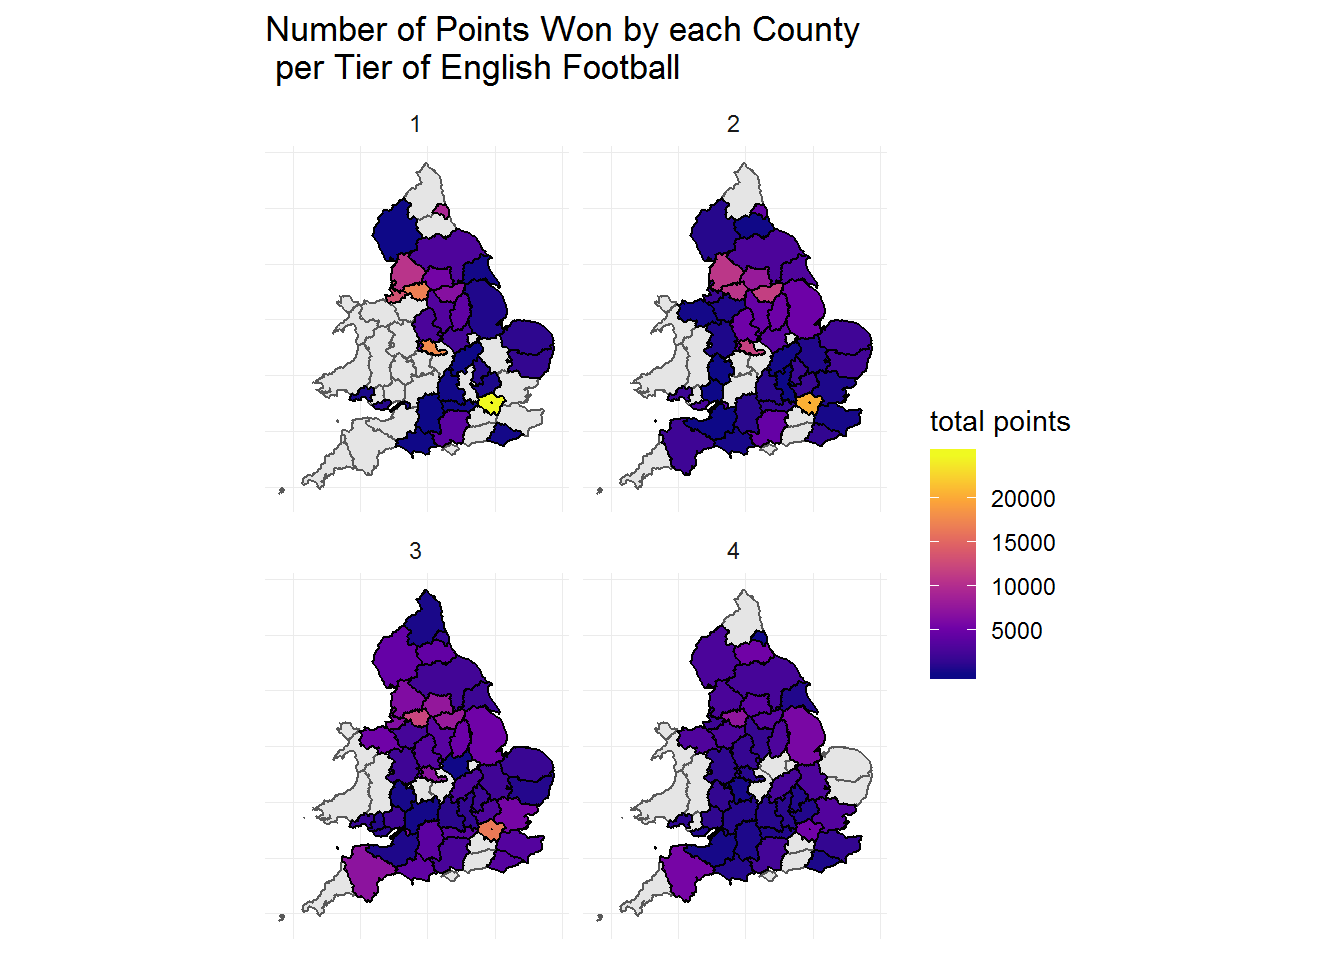
\includegraphics{2019-06-20-The_Knowledge_4_files/figure-latex/unnamed-chunk-2-1.pdf}


\end{document}
